\section{Algorithmic Framework}
\label{af:intro}

This thesis was implemented in Java, using the code from \citet{Teflioudi2011} as base for the top-down ILP
algorithm, on which we added the changes in the refinement step mentioned at Section~\ref{sec:incorporation}. Also, we
change the knowledge base back-end to RDF3X, in order to improve the SPARQL queries performance.

\subsection{Knowledge Base Back-end}

For storing and retrieving RDF data we use RDF3X \citep{Neumann:2010:RES:1731351.1731354}. It has the advantage of being
specialized and optimized for RDF triples, using a strong indexing approach with compressed B$^+$-Tree indices for all
the six permutations of \emph{subject (S)}, \emph{predicate (P)} and \emph{object (O)}:
\emph{SPO},\emph{SOP},\emph{OSP},\emph{OPS},\emph{PSO} and \emph{POS}.

All the facts are stored in a single triples table, with no schema, over which the indices are created. Other six
additional aggregated indices, for each of the pairs of \emph{subject}, \emph{predicate} and \emph{object}
(\emph{SP},\emph{SO},\emph{OS},\emph{OP},\emph{PS} and \emph{PO}), are also created. These indices store only two of the
three columns of a triple and contain an aggregated count for the number of occurrences of the given pair of arguments
among all the triples.

Moreover, all the literals in the facts table are replaced by ids using a mapping dictionary. This brings two important
benefits: the compression of the facts table; and the simplification for the query processor, which is required to
compare ids instead of eventually long strings. Because of that, it also requires two additional indices, one that maps
literals to ids, and another that maps ids to strings.

The query processor explores the exhaustive indexation by relying mostly on merge-joins over the sorted index lists, and
building operator trees that preserve a convenient ordering which allows further merge-joins. When not possible,
RDF3X simply switches to hash-join.

RDF3X supports SPARQL queries, nevertheless, in the version 0.3.7 which was used in this thesis, many features of the
query language were not implement. For example, optional patterns are not supported, and sorting and filtering
operators for numerical attributes is not implemented, with numbers being dealt as strings. The expression $31>4$,
for example, is evaluated as the comparison of strings ``31''$>$``4'', which returns false instead of true. As the
evaluation of numerical expressions plays a key role in this thesis, we had to make changes to the original code
to implement this feature.


\subsection{Correlation Lattice Data Structure}

We structure the correlation lattice data in two main classes: \emph{CorrelationLattice} and
\emph{CorrelationLatticeNode}. 

Basically, in the \emph{CorrelationLattice} class, we store attributes related to the lattice as
a whole, such as the root property, root node, maximum number of levels, as well as attributes consistent through all
the lattice nodes, such as discretization boundaries, support and interestingness thresholds. Moreover, it maintains a
hash set with all the lattice nodes in order to avoid duplicate nodes.

In the \emph{CorrelationLatticeNode} class, we simply store the histogram data obtained with the discretization on
root's numerical attribute, the pointers to the child nodes, the suggestion maps (presented in
Section~\ref{sec:queryingTheLattice}). The UML Class diagram from Figure~\ref{fig:classDiagram} shows in more details
how both classes are structured.

\begin{figure}
\caption{UML Class diagram from CorrelationLattice and CorrelationLatticeNode}
\begin{center}
  \begin{tikzpicture}
    \umlclass[x=2,y=7]{CorrelationLattice} {
	numericalProperty : Property \\
	maximumDepth : Integer \\
	numberOfBuckets : Integer \\
	discretizationBoundaries : Integer[numberOfBuckets-1] \\
	minSupport : Integer \\\
    }{
	saerchRules(minConf, minSupport, minGain) : Set<Rule>\\
    }
    \umlclass[x=2,y=0]{CorrelationLatticeNode} {
      children : CorrelationLatticeNode[] \\
      clause : Literal[] \\
      suggestions : Map<Literal,SortedList<Literal$>>$ \\
      histogram : Integer[] \\
      distribution : Float[] \\
    }{
      getSuggestions(head : Literal) : SortedList<Literal>\\
      search(literal : Literal) : CorrelationLatticeNode\\
    }
    \umlassoc[arg1=lattice, mult1=1, arg2=nodes, mult2=1..*]{CorrelationLattice}{CorrelationLatticeNode} 
  \end{tikzpicture}
\label{fig:classDiagram}
\end{center}
\end{figure}


\subsection{Querying the Correlation Lattice Histograms}

For building the correlation lattice, we start with the root node, which has a numerical property as literal and no
constants assigned, e.g. \emph{hasIncome(X,Y)}. We use the SPARQL query below in order to obtain the  distribution of 
examples along the numerical attribute $Y$ in the whole Knowledge Base.

\begin{center}
 \emph{SELECT COUNT ?Y WHERE \{ ?X <hasIncome> ?Y \} GROUP BY (?Y)}
\end{center}

We also use the result of this query in order to obtain the minimum and maximum values from $Y$, and set the
discretization boundaries for the specified discretization technique. As a result, we can extract the root
node's frequency histogram. We keep the discretization boundaries in the CorrelationLattice class, as it will be used
consistently throughout the whole lattice.

Afterwards, we select the categorical properties that will be used in the lattice. For each of the selected
properties, we join them with the root numerical property, then query the resulting distribution. We extract the node's
histogram for each categorical constant of given property with a single SPARQL query, which is illustrated below for the
categorical relation \emph{hasEducation}:

\begin{center}
 \emph{SELECT COUNT ?Z ?Y WHERE \{ ?X <hasIncome> ?Y . ?X <hasEducation> ?Z \} GROUP BY (?Z,?Y)}
\end{center}

For the further levels, we simply add a pattern correspondent to each literal in the node, querying a combination of
categories individually. For instance, if we combine the categories $hasEducation(X,phd)$ and $hasSex(X,female)$, the
correspondent query would be:

\begin{center}
 \emph{SELECT COUNT ?Y WHERE \{ ?X <hasIncome> ?Y . ?X <hasEducation> <phd> . ?X <hasSex> <female> \} GROUP BY (?Y)}
\end{center}

With these three types of queries and a numerical, we can extract the data required for the frequency histogram of any
node in the lattice.




% Substitution for constants only in categorical relations, query by support
% When categorical joined to numerical property (without range) existent in \graphname query graph for constants
% 



